.

\todo[inline]{Crunch the text!}

Tageted towards caches and eDRAM.

Our goal is to refresh only the data that will be used in the near future, and only refresh if it is really needed. The other data is invalidated and/ or written back to main memory.

The technique target to minimize the refresh for the so called hot and cold lines. Hot lines are those being accessed and thus unnesssesary refreshed by the refresh mechanism, whereas the cold lines are those that hasn't been used in a while but still gets refreshed.

To minimize the refresh for hot lines time-based policies are used. Normally a counter - Polyphase - is used, which practicly works in the same way as the time-out counters for Smart Refresh. It consists of two bits. They also has a basic periodic refresh scheme (why?).

For the cold lines four different (data-based) policies can be applied: \textit{all}, \textit{valid}, \textit{dirty} or WB(n,m). \textit{All} refreshes all lines. \textit{Valid} refreshes the valid lines. \textit{Dirty} refreshes the dirty lines. The WB policy is associated with a tuple (n, m). WB refreshes a Dirty line that is not being accessed for n times before writing it back and changing its state to Valid Clean; moreover, it refreshes a Valid Clean line that is not being accessed for m times before invalidating it. WB retains a Dirty line in the cache Ion ger because evicting it has the additional cost of writing the line back to lower-Ievel memory. To implement WB, we maintain a per-Iine Count. W hen the line is read or written, Count is set to n (if Dirty) or m (if Valid Clean). In addition, when the line is refreshed, Count is decremented. W hen Count reaches zero, the line is either written back or invalidated. Note that the Dirty policy is equivalent to WB(oo,O), while Valid is equivalent to WB(oo,oo). Finally, every policy refreshes cache lines in transient states as well.

They categorize applications based on how they are affected by the data-based policies. Fig. \ref{fig:app_cat} presents an application categorization based on two axes: application footprint and visibility. It is likely........ TODO

\begin{figure}[t!]
	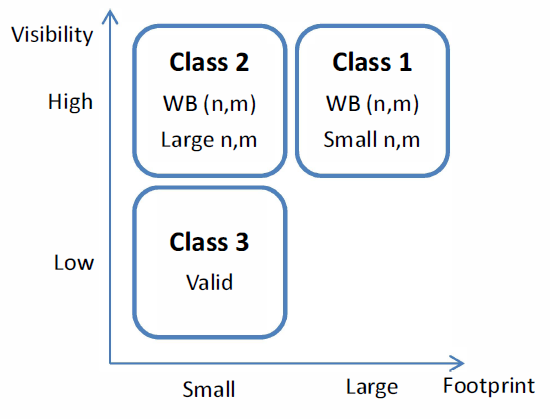
\includegraphics[width=\textwidth/2]{app_cat}
	\caption{Application categorization according to the data-based policy \cite{refrint}.}
	\label{fig:app_cat}
\end{figure}

Implementation: Hot lines. They use a global counter with M bits (M = 1 or 2). When a line is accessed, the global counter is copied to N bits associated to the line and those N bits are stored with the valid bit in the memory controller. If N = 2, the overhead becomes 0.6\%. When the global counter steps to a new phase, all normal accesses are stalled and the logic controlls the valid lines and its local phase bits to see if it matches the global phase. If there is a match, a refresh is scheduled. Otherwise the memory goes back to normal operation after the scan. 

Implementation: Cold lines. For each line there is a 5 bit counter and the line's state bits. Depending on the data policy  for each line, but they are somehow neglectible.  ...

Remember that this technique is targeted towards caches and eDRAM and only is tested in that enviroment. This means that we can not really use the results shown in their paper, but the techniques can be applied to DRAM.

\subsubsection*{Differences and similarities}

Refrint is somewhat a extension of Smart Refresh. Smart Refresh's features can be laid somewhat equal to Refrint's time-based polices, wheras the data-based polices have no eqvivalence in Smart Refresh.

They both modify the memory controller, and almost in the same way. But Refrint has no timers that is getting decremented the whole time, and instead copies a global "timer" to the line associated bits upon access. Of cource Refrint's data-based polices also adds logic to the memory controller.

Discuss energy savings. Hard to do eDRAM vs DRAM...

